%system developement

Study of parameters affecting short circuit capacity of the circuit breaker is divided in:
\begin{enumerate}
\item Modeling of system for TRV studies under different fault conditions
\item Modeling of system under different fault conditions for arc interruption studies
\item Measurement of Dynamic Contact Resistance of CBs and analysis of collected DCRM signature data
\end{enumerate}

\section{Computational Models}
\subsection{Interruption of Three Phase to Ground fault}
A model of IEEE network is developed in EMTP-RV. As shown in figure \ref{fig:IEEE Network under Study }, the system consists of local sources and remote sources connected through transmission lines. Four transmission lines and two transformers supply the 145 kV station. Details are shown in figure \ref{fig:IEEE Network under Study }. Stray capacitances of equipments are also considered. The system is studied for Three Phase to Ground fault at the terminal of station for multiple lines switching and transformer switching. Breaker rating of 30 kA maximum current interruption capacity is selected for the study. Current in the steady state through fault is found out. Accordingly standard TRV is built. TRV through simulation is compared with standard TRV provided by application guide. The ability of fault interruption capability of CB is found out.

\subsection{Interruption of Single  Phase to Ground fault}
The network is further studied for Single Phase to Ground short line fault at 4.2 km from station for 16 km line. The lines are modeled in constant parameter mode as well as frequency dependent mode TRV through simulation is compared with standard TRV provided by application guide for both frequency dependent and constant parameter line model. The ability of fault interruption capability of CB is found out.

\begin{figure}[!htbp]
    \centering
    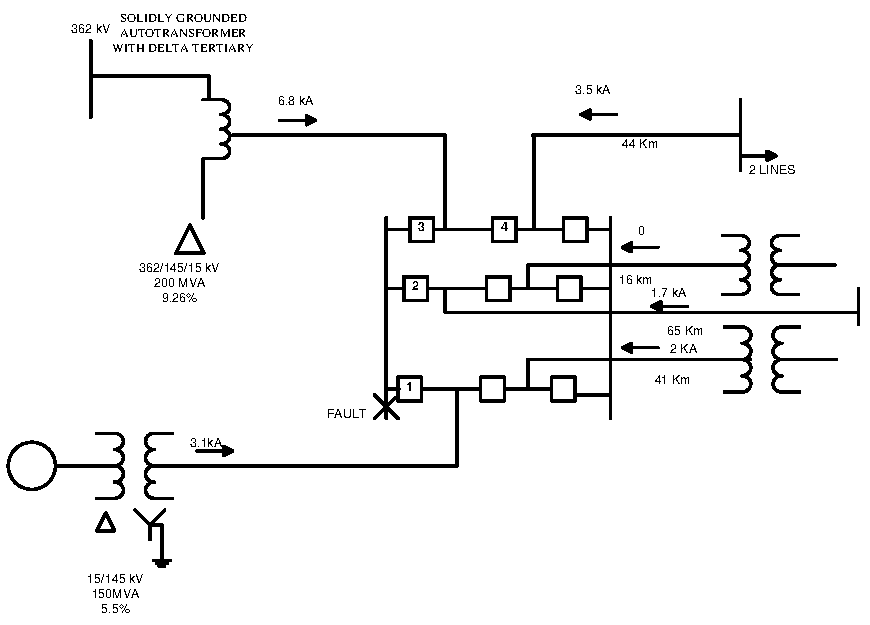
\includegraphics[width=\textwidth]{onelinediagram}
    \caption[IEEE Network under Study]{IEEE Network under Study \cite{ApplicationofTransientRecovery}}
    \label{fig:IEEE Network under Study }
\end{figure}

\subsubsection*{Parameters of the model}

\textbf{1. Local Source 1}\\
L-L RMS Voltage - 362 kV\\
Resistance - 0.16 $\Omega$\\
Inductive Reactance - 16.2 $\Omega$\\
\clearpage

\textbf{2. Transformer}\\
Nominal Rating - 200 MVA\\
L-L RMS Primary Voltage - 362 kV \\
L-L RMS Secondary Voltage - 145 kV\\
Connection type - Yg-Yg\\
Winding Resistance - 0.0009 pu\\
Winding Reactance - 0.0926 pu\\

\textbf{3. Generator Transformer}\\
Nominal Rating - 150 MVA\\
L-L RMS Primary Voltage - 15 kV \\
L-L RMS Secondary Voltage - 145 kV\\
Connection type - DYg+\ang{30}\\
Winding Resistance - 0.0005 pu\\
Winding Reactance - 0.055 pu\\

\textbf{4. Local Source 2}\\
L-L RMS Primary Voltage - 15 kV\\
Resistance - 0.002 $\Omega$\\
Inductive Reactance - 0.209 $\Omega$\\

\textbf{5. Transmission Line}\\
L-L RMS Voltage - 145 kV\\
Positive Sequence Resistance - 0.01$\Omega$\\
Zero Sequence Resistance - 0.1 $\Omega$\\
Positive Sequence Surge Impedance - 350 $\Omega$\\
Zero Sequence Resistance - 560 $\Omega$\\
Propagation Speed - 1.9 $\times$ 105 m/s\\
Length of lines - 44 km, 16 km, 65 km , 41 km\\

\clearpage

\textbf{6. Parameters of lines for frequency dependent model}\\

\begin{tabular}{ | >{\centering\arraybackslash}m{0.7in} | >{\centering\arraybackslash}m{0.7in} | >{\centering\arraybackslash}m{0.7in} | >{\centering\arraybackslash}m{0.7in} | >{\centering\arraybackslash}m{0.7in} | >{\centering\arraybackslash}m{1.2in} |} \hline
Phase & DC resistance & Outside diameter & Horizontal distance & Vertical distance &	Vertical distance at mid span  \\
{~} & $\Omega$ & (m)& (m)& (m)& (m) \\ \hline
1	& 0.126 & 0.12	&-8	&	20	&	20 \\ \hline
2	& 0.126	&0.12	&0	&	20	&	20 \\ \hline
3	& 0.126	&0.12	&8	&	20	&	20 \\ \hline
0	& 3		&0.08	&-6	&	26	&	26 \\ \hline
0	& 3		&0.08	&6	&	26	&	26 \\ \hline
\end{tabular}

~\\
\textbf{7. Arc parameters}\\
$\tau_m$ = 0.5 E-06\\
$P_0$ = 10.0 E+04\\
$\tau_c$ = 1E-06\\
$U_C$ = 2000\\
$g_0$ = 5E+07\\
$t_{trip}$ = 20 E-03\\

\section{Analytical Models}

\subsection{Transient Recovery Voltage types}
Three phase terminal fault is the most severe fault used to define the breaker rating. However, for the transmission voltages, the probability of occurrence of three phase terminal fault is very low. Hence the three phase to ground faults are the basis for rating the CB. Short line faults have lower crest magnitudes, but they have high RRRV.

\subsubsection{Three phase terminal fault}
The circuit showed in Figure \ref{fig:Circuit for Interruption of a Three-Phase-to-Ground Fault} defines the electrical equivalent network for the first phase to clear during the interruption of a three-phase terminal fault. The corresponding one-line diagram representation is shown in Figure \ref{fig:Single Line Diagram}, while Figure \ref{fig:Three Phase Diagram} indicates the three-phase representation. The reduced simple parallel RLC circuit is shown in the equivalent circuit given by Figure \ref{fig:Equivalent Circuit}. The equivalent components are given by

Equivalent inductance
\begin{equation}\label{eq:3.1}
L_{eq} = \frac{3 L_0 L_1}{L_1 + 2 L_0}
\end{equation}

In effectively grounded systems, for three-phase-to-ground faults \textit{i.e.}, with first pole-to-clear factor equal to 1.3; $L_{eq} = 1.3 L_1$.

In ungrounded systems ($L_0$ infinite), for three-phase-to-ground faults \textit{i.e.}, with first-pole-to-clear factor equal to 1.5; $L_{eq} = 1.5 L_1$

Equivalent surge impedance
\begin{equation}\label{eq:3.2}
Z_{eq} = \frac{3}{n} \times \frac{Z_0 Z_1}{Z_1 + 2 Z_0}
\end{equation}
where\\
$Z_0 = 1.6 Z_1$\\
$Z_{eq} = 1.14 Z_1 / n $\\

Equivalent capacitance
\begin{equation}\label{eq:3.3}
C_{eq} = \frac{C_0 + 2 C_1}{3}
\end{equation}

where\\
$Z_1$ - positive-sequence surge impedance of the transmission lines\\
$Z_0$ - zero-sequence surge impedance of the transmission lines \\
$n$ - number of lines\\
$L_1$- positive-sequence inductance, of all other parallel sources terminating at the station \\
$L_0$ - zero-sequence inductance, of all other parallel sources terminating at the station\\
$C_1$ - positive-sequence capacitance\\
$C_0$ - zero-sequence capacitance

For three-phase ungrounded faults on effectively grounded systems:\\
$L_{eq} = 1.5 L_1$; $Z_{eq} = 1.5 Z_1 / n$; $C_eq = C_1 / 1.5$\\

\begin{figure}
    \centering
    \begin{subfigure}[b]{\textwidth}
        \centering
        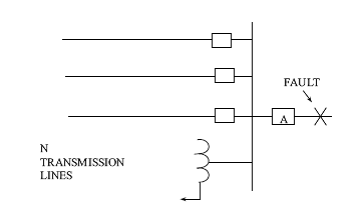
\includegraphics{f1SingleLineDiagram}
        \caption{Single Line Diagram}
        \label{fig:Single Line Diagram}
    \end{subfigure}
    
    \begin{subfigure}[b]{\textwidth}
        \centering
        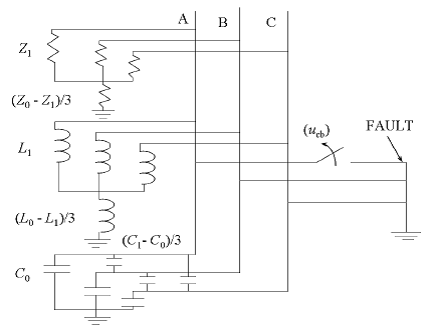
\includegraphics{f2ThreePhaseDiagram}
        \caption{Three Phase Diagram}
        \label{fig:Three Phase Diagram}
    \end{subfigure}

    \begin{subfigure}[b]{\textwidth}
        \centering
        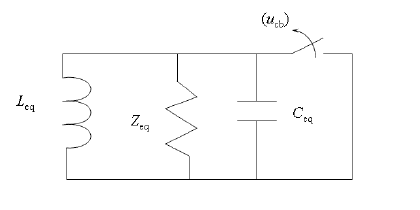
\includegraphics{f3EquivalentCircuitn}
        \caption{Equivalent Circuit}
        \label{fig:Equivalent Circuit}
    \end{subfigure}
    \caption{Circuit for Interruption of a Three-Phase-to-Ground Fault}
    \label{fig:Circuit for Interruption of a Three-Phase-to-Ground Fault}
\end{figure}

\subsubsection{Exponential (Overdamped) TRV}
The TRV across the CB contacts can be found using current injection technique as the time span is short (microseconds). The current can be represented by a ramp. The solution for the parallel RLC network shown in Figure \ref{fig:Equivalent Circuit} is given by Equation (\ref{eq:3.4}):

\begin{equation}\label{eq:3.4}
u_{cb} = u_1 \left( 1 - e^{\alpha t} \left( \cosh \beta t + \frac{\alpha}{\beta} \sinh \beta t \right) \right) kV
\end{equation}

$u_{cb}$ =  voltage across the open circuit-breaker contacts\\
$u_1 = \sqrt{2} I \omega L_{eq}, (kV)$\\
$\omega = 2 \Pi f, (rad/s)$\\
$I$ = rms value short-circuit current, (kA)\\
$\alpha = \frac{1}{2 Z_{eq} C_{eq}}$\\
$\beta =\sqrt{\alpha^2 - \frac{1}{(L_{eq} C_{eq})}}$\\
$Z_{eq}$ - equivalent impedance ($\Omega$)\\
$L_{eq}$ - equivalent inductance ($H$)\\
$C_{eq}$ - equivalent capacitance ($F$)\\

In most of the applications, the parallel resistance of the line surge impedances of the lines is such that it effectively swamps the capacitance of the circuit. Hence it is a common practice to neglect the capacitance. The solution to the simple RL circuit is given by equation (\ref{eq:3.5}):

\begin{equation}\label{eq:3.5}
u_{cb} = u_1 \left( 1 - e^{-t / \tau} \right) kV
\end{equation}
where\\
$\tau = \frac{L_{eq}}{Z_{eq}} s$

\subsubsection[Single frequency recovery voltage]{Single frequency recovery voltage\\(Oscillatory underdamped TRV)}
When the short circuit is fed by a transformer and numbers of lines remain connected to the bus, the resulting TRV is oscillatory single frequency TRV. Figure \ref{fig:Equivalent Circuit} shows the equivalent circuit with resistance removed. The circuit becomes underdamped and the response is a typical 1-cosine waveform. Equation \ref{eq:3.6} is the approximate equation for the voltage across the open circuit breaker contacts of CB.

\begin{equation}\label{eq:3.6}
u_{cb} = u_1 \left[ 1 - \cos \left( \frac{t}{\sqrt{L_{eq} C_{eq}}} \right) \right]
\end{equation}

\subsection{Traveling waves}
The transmission line can be represented as an inductive elements connected in series and capacitive elements distributed along the line in parallel. The voltage applied at one end travels as an electromagnetic wave with the speed of light. When the transmitted wave reaches discontinuity, the wave gets reflected and refracted depending on the discontinuity. The time for the wave to go out from the discontinuity and back is given by:

\begin{equation}\label{eq:3.7}
T = 6.68 l \sqrt{\mu \epsilon} ~~\mu s
\end{equation}

$l$ - distance to the first discontinuity (km)\\
$\mu$ - magnetic permeability\\
$\epsilon$ - dielectric constant

The coefficients for the new voltage waves are\\
\begin{equation}\label{eq:3.8}
\text{Reflection,~~~} K_R = \frac{Z_2 - Z_1}{Z_2 + Z_1}
\end{equation}
\begin{equation}\label{eq:3.9}
\text{Refraction,~~~} K_T = \frac{2 Z_2}{Z_2 + Z_1}
\end{equation}
$Z_1$ and $Z_2$ are the surge impedances on either side of the discontinuity.

\subsection{Short Line Fault}
The TRV across the CB contacts after the interruption of short line fault consists of the voltage generated by the supply network and of the voltage created by the line side oscillation. Due to distributed constants of the transmission line, the line side oscillations are in the form of traveling waves. The reflection of this traveling wave against the short circuit point and the open end at the breaker side cause a triangular shaped waveform.

The travel time of the electromagnetic waves in case of single line to ground fault at a distance \textquoteleft$l$\textquoteright ~from the breaker to the fault location is given by
\[
\tau_{Line} = \frac{l}{\vartheta}
\]
Where $\vartheta$ is the wave velocity that depends on the transmission line parameters. The wave reflected by the short circuit point arrives at the open end near the breaker after twice the travel time. The lattice diagram shown in figure \ref{fig:Lattice Diagram to Evaluate the Characteristics of Travelling Wave} is used to evaluate the characteristics of travelling wave for short line fault. The numerical value of the coefficients for the reflected and transmitted wave shows the amplitude multiplier for the voltage wave. Single phase circuit for short line fault with source ($X_S$) and the line reactance ( $\lambda * X_L$ ) is shown in figure \ref{fig:Single-Phase Circuit with Short-Line Fault}. The fault current is given by equation \ref{eq:3.10}.

\begin{equation}\label{eq:3.10}
I_L = \frac{u_{LG}}{\lambda \times X_L + X_s}
\end{equation}
$X_L$ - reactance of the line to the fault point per kilometer, given by $\frac{(2L_{1 \omega} + L_{0 \omega})\omega}{3}$\\
$L_1$ - positive sequence power-frequency line inductance per kilometer\\
$L_0$ - zero sequence power-frequency line inductance per kilometer\\
$u_{LG}$ - line to ground system voltage (kV)\\
$\lambda$ - distance of CB to the fault (km)\\
$I_L$ - terminal fault current (kA)

\begin{equation}\label{eq:3.11}
\frac{d u_L}{dt} = \sqrt{2} \omega I_L Z_{eff}
\end{equation}

\begin{figure}[!htbp]
    \centering
    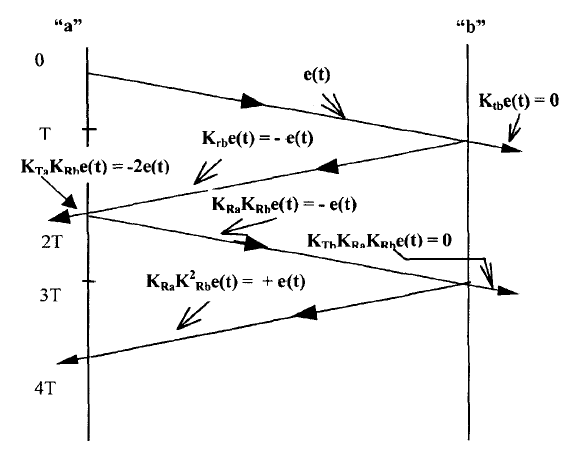
\includegraphics[width=\textwidth]{LatticeDiagramtoEvaluatetheCharacteristicsofTravellingWave}
    \caption{Lattice Diagram to Evaluate the Characteristics of Travelling Wave}
    \label{fig:Lattice Diagram to Evaluate the Characteristics of Travelling Wave}
\end{figure}

\begin{figure}
    \centering
    \begin{subfigure}[b]{0.5\textwidth}
        \centering
        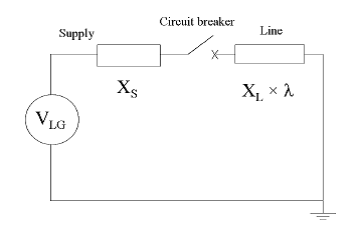
\includegraphics[width=\textwidth]{g1SinglePhaseCircuitwith}
        \caption{Single-Phase Circuit with Short-Line Fault}
        \label{fig:Single-Phase Circuit with Short-Line Fault}
    \end{subfigure}
    \\
    \begin{subfigure}[b]{0.49\textwidth}
        \centering
        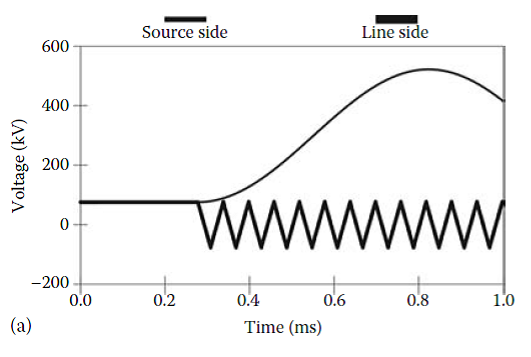
\includegraphics[width=\textwidth]{g2LineSideandSourceSideVoltages}
        \caption{Line Side and Source Side Voltages}
        \label{fig:Line Side and Source Side Voltages}
    \end{subfigure}
    \begin{subfigure}[b]{0.49\textwidth}
        \centering
        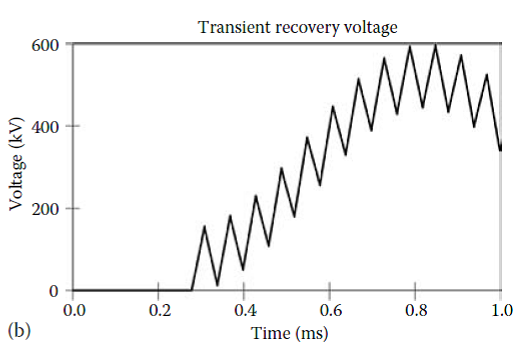
\includegraphics[width=\textwidth]{g3TransientRecoveryVoltage}
        \caption{Transient Recovery Voltage}
        \label{fig:Transient Recovery Voltage}
    \end{subfigure}
    \caption{TRV across the Breaker during Short Line Fault}
    \label{fig:TRV across the Breaker during Short Line Fault}
\end{figure}
The source side and line side TRV shapes during short line fault is shown in figure \ref{fig:TRV across the Breaker during Short Line Fault}.

\clearpage
\section{Mathematical Model}
Configuration of contacts plays a crucial role in the performance of CB. Contact resistance depends on the contact forces and the actual contact area. The contact resistance is given by

\begin{equation}
R_T = \frac{\rho}{2} \sqrt{\frac{\pi K H }{F_T}} + R_F
\end{equation}

Where:\\
$H$ - Material hardness\\
$K$ - Constant between 0.1 and 0.3\\
$\rho$  - Resistivity of contact material\\
$R_F$ - Film resistance\\
$F_T$ - Total force acting on a contact
The current get constricted at the point of contact. This constriction of current is responsible for contact resistance and the heat generated at the contacts. It is also the source of electromagnetic force that acts upon contact structure.

For a circular cluster contacts, three forces act upon: the attractive force ($F_A$), repulsive force ($F_R$) and contact spring force ($F_S$). Thus the total force ($F_T$) acting on a contact is given by 

\begin{equation}
F_T = F_S + F_R - F_A
\end{equation}

The attraction force should be greater than the repulsive force for a CB contacts. When SF\textsubscript{6} CB contacts are subjected to arcing, a sulfide coat is formed. This sulfide coat increases the contact resistance if there is no scrapping or wiping motion between the contacts. The sulfide coat gets removed by slight friction and decomposed by heat. The force of attraction exists between two opposite fingers of a circular cluster contacts when current is flowing in the same direction. This force of attraction for contact having \textquoteleft$n$\textquoteright ~ fingers and distance \textquoteleft$d$\textquoteright ~between fingers with a current of $I/n$ through each finger is given by 

\begin{equation}
F_A = 0.102 (n-1) \left( \frac{I}{n}\right)^2 \left( \frac{l}{d}\right)
\end{equation}

The attractive force pinches the moving contact fingers on the fixed contact which reduces the contact resistance as shown in Fig 3.3.1. The wiping action on the contacts get improved which helps in removing the sulfide coat \cite{hedman2009optimal}. The CB contacts should be properly designed for wiping action so that the problem of metallic fluoride deposition is minimized \cite{kezunovic2014reliable}.

\begin{figure}[!htbp]
    \centering
    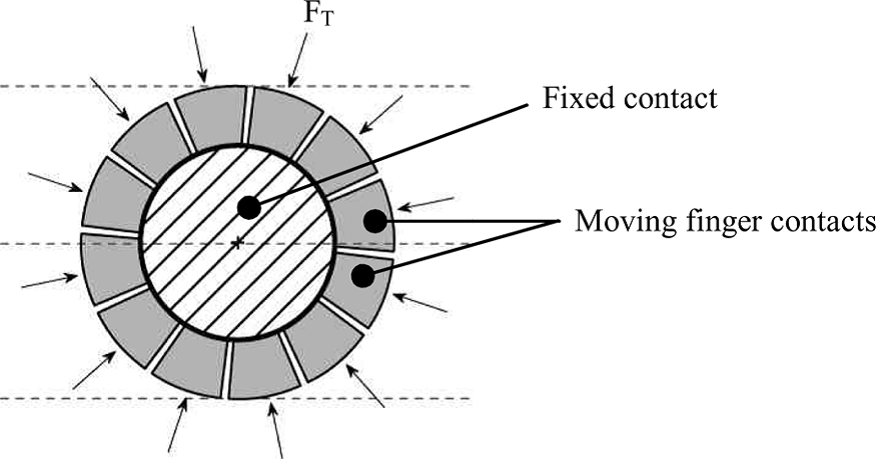
\includegraphics[width=\textwidth]{SchematicofForcesExertedontheFixed}
    \caption{Schematic of Forces Exerted on the Fixed Contact by the Moving Finger Contacts}
    \label{fig:Schematic of Forces Exerted on the Fixed Contact by the Moving Finger Contacts}
\end{figure}

CB is an electromechanical device. Hence its model is governed by mechanical and electromagnetic equations. Mechanical equation of a CB is expressed by the Newton's second law, as shown in equation \ref{eq:3.17}

\begin{equation}\label{eq:3.17}
\rho \left( \frac{\partial^2 u}{\partial t^2} \right) =  \nabla \cdot FS + F_v
\end{equation}
$F_v$ - force per unit volume of deformed mass (N)\\
$\rho$ - mass density ($kg/m^3$)\\ 
$S$ - second order Piola-Kirchhoff stress\\
$F$ - deformation gradient\\
$U$ - mechanical displacement (m) 

Electromagnetic equations of CB are expressed by (\ref{eq:3.18})-(\ref{eq:3.22})

\begin{equation}\label{eq:3.18}
J = \sigma E + J_e
\end{equation}
\begin{equation}
E = - \nabla V
\end{equation}
\begin{equation}
\nabla \cdot J = Q_j
\end{equation}
\begin{equation}
\nabla \times (\mu \nabla \times A_z) = J
\end{equation}
\begin{equation} \label{eq:3.22}
F = J \times B
\end{equation}

$\sigma$ - electrical conductivity $(S/m)$\\
$J_e$ - applied current density $(A/m^2)$\\ 
$J$ - current density $(A/m^2)$\\ 
$V$ - voltage (V) \\
$E$ - electric field $(V/m)$ \\
$Q_j$ - charge per unit volume $(C/m^3)$\\
$\mu$ - average permeability\\
$A_z$ - magnetic vector potential\\
$B$ - magnetic field in Tesla \\
$F$ - magnetic force of the Lorentz law (N)

Passage of electricity produces heat, and this heat affects the resistance and electrical and mechanical properties of CB. 

\subsection{Contact resistance measurement method}
Standard Timing test is performed on breaker followed by static contact resistance measurement. Figure \ref{fig:Schematic Diagram of Static Contact Resistance Measurement} shows the arrangement for static contact resistance measurement. The value of test current should be as per the manufactures specifications. IEC and ANSI recommend 50 A and 100 A respectively. Breaker is kept in closed position. 100 A DC current is passed through the contacts. Voltage drop is measured and contact resistance is calculated.

\begin{figure}[!htbp]
    \centering
    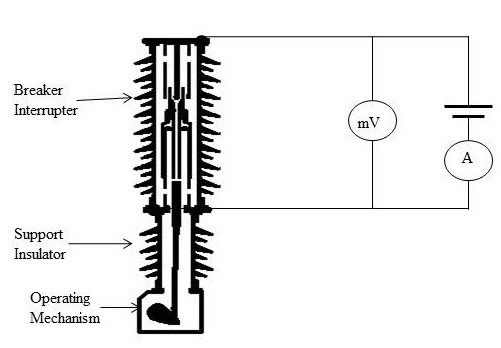
\includegraphics[width=\textwidth]{SchematicDiagramofStaticContactResistanceMeasurement}
    \caption{Schematic Diagram of Static Contact Resistance Measurement}
    \label{fig:Schematic Diagram of Static Contact Resistance Measurement}
\end{figure}

\begin{figure}[!htbp]
    \centering
    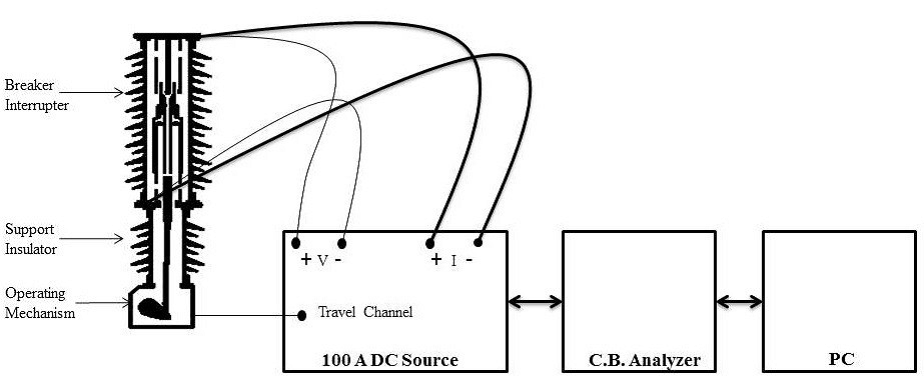
\includegraphics[width=\textwidth]{SchematicDiagramofDCRM}
    \caption{Schematic Diagram of DCRM}
    \label{fig:Schematic Diagram of DCRM}
\end{figure}

The schematic diagram of DCRM is shown in figure \ref{fig:Schematic Diagram of DCRM}. The close-trip command is given to CB. 100A DC current is injected, and the CB is operated at rated speed. Depending on the breaker technology, linear or rotary contact travel transducer is used for recording contact movement. The instantaneous value of resistance is measured along with contact travel. The test kit of Scope Company with Hisac Ultima test manager software for analysis is used. Measuring system with a sampling frequency of 10 kHz and 100 $\mu s$ resolution is used to record the resistance with precision as well as to record the transfer of current from arcing contact to the main contact and vice-versa. A time delay of 300 ms is kept between close-trip operations. The test set up is connected to a portable computer for calculation of instantaneous contact resistance, data analysis and interpretation using the software. The variations in the resistance over time are recorded as a finger print for the breaker contacts. This recorded signature can be used as a benchmark for comparison of the future measurement record of the same breaker. The DCRM signature provides information on the breaker contacts and the operating mechanism. Measuring system and test set up is shown in Figure \ref{fig:Test set up for DCR Measurement}.

\begin{figure}
    \centering
    \begin{subfigure}[b]{0.49\textwidth}
        \centering
        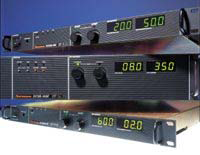
\includegraphics[width=\textwidth]{h1Stablecurrentsource}
        \caption{Stable Current Source}
        \label{fig:Stable current source}
    \end{subfigure}
    \\
    \begin{subfigure}[b]{0.49\textwidth}
        \centering
        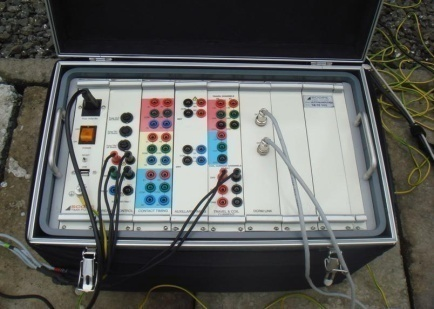
\includegraphics[width=\textwidth, height = 5cm]{h2Dataacquisitionsystem}
        \caption{Data Acquisition System}
        \label{fig:Data acquisition system}
    \end{subfigure}
    \begin{subfigure}[b]{0.49\textwidth}
        \centering
        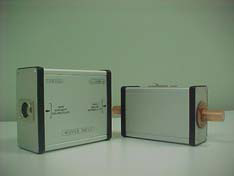
\includegraphics[width=\textwidth, height = 5cm]{h3VoltageandCurrentsensors}
        \caption{Voltage and Current Sensors}
        \label{fig:Voltage and Current sensors}
    \end{subfigure}
    \\
    \begin{subfigure}[b]{0.49\textwidth}
        \centering
        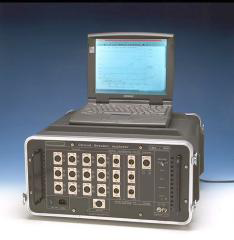
\includegraphics[width=\textwidth]{h4Testmanagersoftware}
        \caption{Test Manager Software}
        \label{fig:Test manager software}
    \end{subfigure}
    \caption{Test Set Up for DCR Measurement}
    \label{fig:Test set up for DCR Measurement}
\end{figure}

\subsection{DCRM signature analysis}
Figure \ref{fig:Measurement Details from DCRM Signature} shows the measurement details from DCRM signature. DCRM may be called as an ECG of the circuit breaker. The analysis software provided with a test kit can be used for analysis. However, analysis of signature needs the knowledge of CB design, interrupter design, operating mechanism and also expertise to detect the problem. Every CB has a different shape of DCRM signature which mainly depends on contact design, type of operating mechanism, contact wipe, contact speed, \textit{etc}. The deviations in the signature can be found by superimposing earlier signature. Parameters such as length of arcing contact, erosion of contacts, mechanical problem, contact travel and speed, healthiness of mechanism, \textit{etc}. can be obtained from the signature. An enlarged view of DCRM signature in the tripping zone is shown in figure \ref{fig:Enlarged View of Tripping Portion of DCRM Signature}.

\begin{figure}[!htbp]
\centering
\begin{minipage}{\textwidth}
\centering
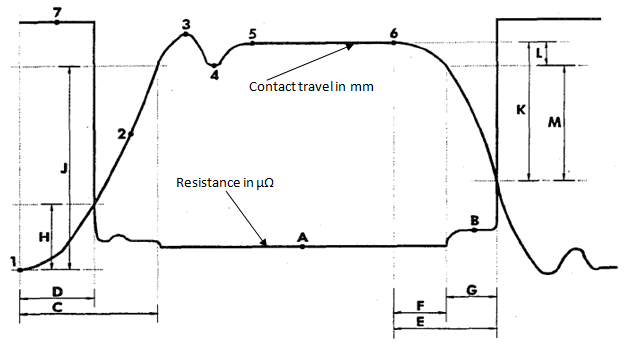
\includegraphics[width=\textwidth]{MeasurementDetailsfromDCRMSignature}
\caption{Measurement Details from DCRM Signature}
\label{fig:Measurement Details from DCRM Signature}
\begin{flushleft}
\footnotesize A: main contact resistance\\
B: arcing contact resistance\\
C: time for main contacts to make\\
D: time for arcing contacts to make\\
E: time for arcing contacts to break\\
F: time for main contacts to break\\
G: time arcing contact made\\
H: distance for arcing contacts to make\\
J: distance for main contacts to make\\
K: distance for arcing contacts to break\\
L: distance for main contacts to break (wipe of main contact)\\
M: distance arcing contacts made (wipe of arcing contact)\\
\end{flushleft}
\end{minipage}
\end{figure}

\begin{figure}[!htbp]
    \centering
    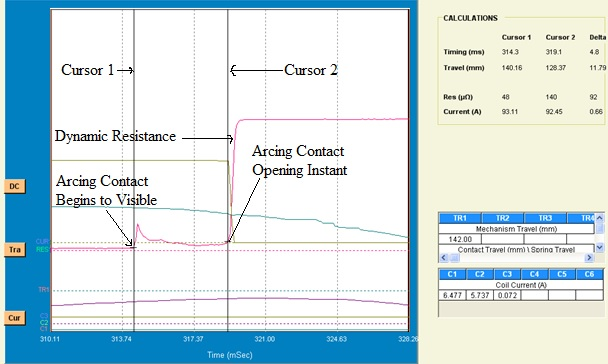
\includegraphics[width=\textwidth]{EnlargedViewofTrippingPortionofDCRMSignature}
    \caption{Enlarged View of Tripping Portion of DCRM Signature}
    \label{fig:Enlarged View of Tripping Portion of DCRM Signature}
\end{figure}

\subsection{Case studies}
POWERGRID and many utility companies in India are using DCRM test for condition assessment of CBs. Case studies from the field are discussed in this section which signifies the use of DCRM signature in detecting the problems at an early stage in CBs.

\subsubsection*{Case no. 1}
Contact bouncing~ for longer duration~ in no load closing characteristics~ at manufacturer works (Figures \ref{fig:Contact Bouncing after Closing Cycle on 400 kV SF6 Circuit Breaker} to \ref{fig:DCRM Signature Showing Fluctuations in Resistance Curve of B Phase Front Side Interrupter}) was seen for a 400 kV SF\textsubscript{6} CB during closing operation. The bouncing was noticed after the completion of mechanical travel. Problem was analyzed in the following steps:

\begin{enumerate}
\item The external connections were verified and were found normal. The connections of the test leads connecting main contacts to analyzer were also checked and found correct. The test was repeated with a different analyzer to rule out the electrical signaling fault. But the same problem persisted. It was then confirmed that the problem is within the interrupter assembly

\item Static contact resistance was measured and found to be very high 120 to 160 k$\Omega$

\item The bouncing in the no load closing characteristics is verified by conducting the DCRM test of a B-phase front side interrupter

\item Lot of fluctuations in the current and resistance curve in the no action zone was observed in the DCRM signature

\item Abnormal DCRM signature for the rear side of the same pole was obtained even though no abnormal contact bouncing was seen in no load closing operation

\item The investigations in subassemblies were done in steps and the cause of the problem was detected in moving contact assembly. The puffer cylinder and cylinder support joint was found loose. During assembly of the interrupter, tightening torque was not applied
\end{enumerate}

\begin{figure}[!htbp]
    \centering
    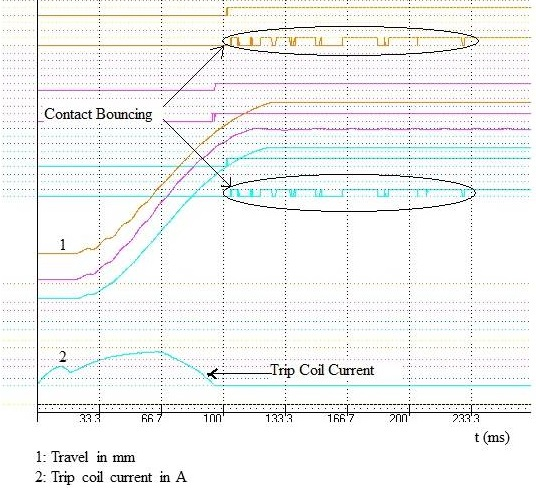
\includegraphics[width=\textwidth]{ContactBouncingafterClosingCycle}
    \caption{Contact Bouncing after Closing Cycle on 400 kV SF\textsubscript{6} Circuit Breaker}
    \label{fig:Contact Bouncing after Closing Cycle on 400 kV SF6 Circuit Breaker}
\end{figure}

\begin{figure}[!htbp]
    \centering
    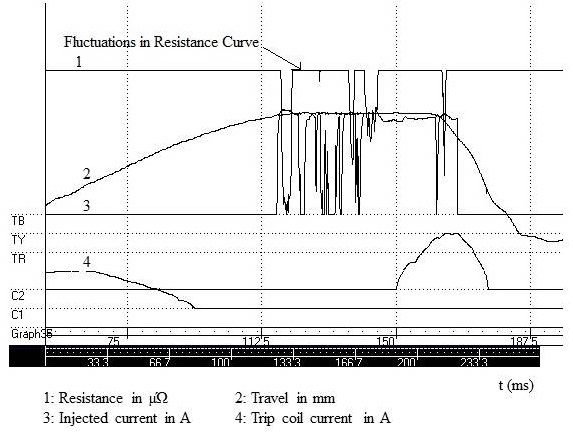
\includegraphics[width=\textwidth]{DCRMSignatureShowingFluctuationsinResistance}
    \caption{DCRM Signature Showing Fluctuations in Resistance Curve of B Phase Front Side Interrupter}
    \label{fig:DCRM Signature Showing Fluctuations in Resistance Curve of B Phase Front Side Interrupter}
\end{figure}

\subsubsection*{Case no. 2}
For a 245 kV SF\textsubscript{6} CB, contact mismatch was observed in the opening operation. The mismatch was not getting adjusted with spring and coil adjustments. The speed time graph was analyzed and following points were noticed:

\begin{enumerate}
\item For R and Y poles, abnormal contact bouncing for more than 5 milliseconds was observed in closing operation

\item As compared to B pole, the wipe was less for R and Y pole in opening operation
\end{enumerate}

The DCRM signatures were obtained for all three phases. The signatures were analyzed for closing and tripping. As seen in the figures \ref{fig:Enlarged View of R-Pole DCRM in Closing Part} and \ref{fig:R-Pole DCRM in Tripping Zone}, abnormality in travel curve and current, as well as resistance, was observed. DCRM of R-pole during tripping can be seen in figure \ref{fig:Y-Pole DCRM in Tripping Zone}. The CB was opened. It was observed that 145 kV arcing contact was fitted instead of 245 kV arcing contact during assembly as seen in figure \ref{fig:Wrong Assembly of Arcing Contact}. DCRM signatures were normal after fitting proper arcing contact.

\begin{figure}[!htbp]
    \centering
    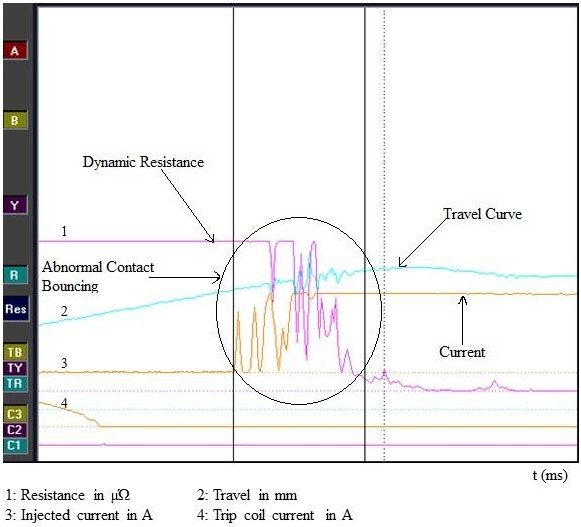
\includegraphics[width=\textwidth]{EnlargedViewofRPoleDCRM}
    \caption{Enlarged View of R-Pole DCRM in Closing Part}
    \label{fig:Enlarged View of R-Pole DCRM in Closing Part}
\end{figure}

\begin{figure}[!htbp]
    \centering
    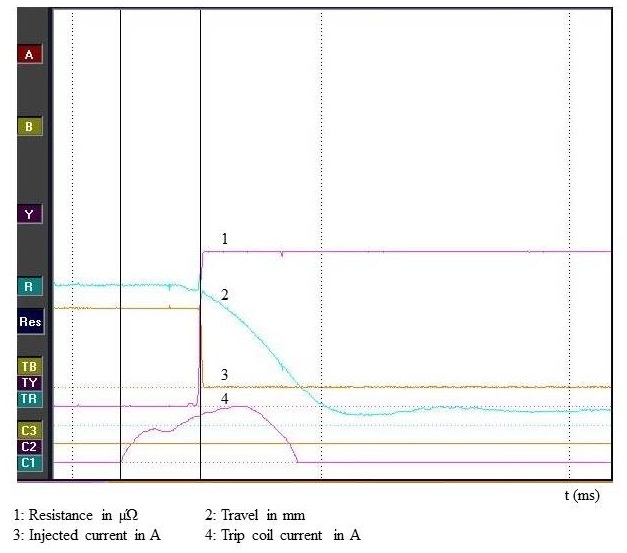
\includegraphics[height=4in]{RPoleDCRMinTrippingZone}
    \caption{R-Pole DCRM in Tripping Zone}
    \label{fig:R-Pole DCRM in Tripping Zone}
\end{figure}

\begin{figure}[!htbp]
    \centering
    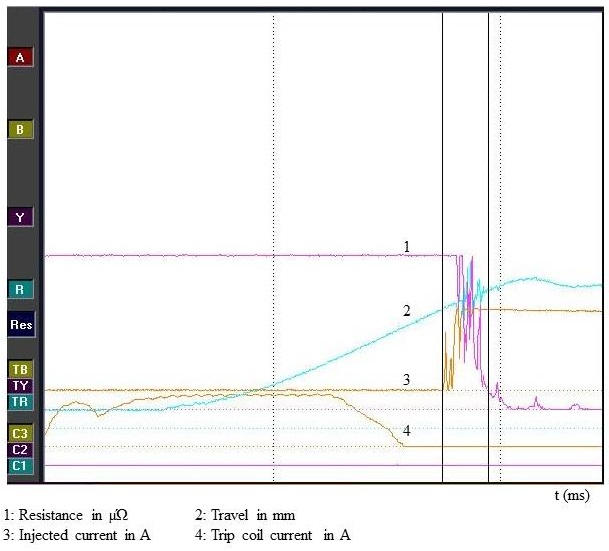
\includegraphics[height=4in]{YPoleDCRMinTrippingZone}
    \caption{Y-Pole DCRM in Tripping Zone}
    \label{fig:Y-Pole DCRM in Tripping Zone}
\end{figure}

\begin{figure}[!htbp]
    \centering
    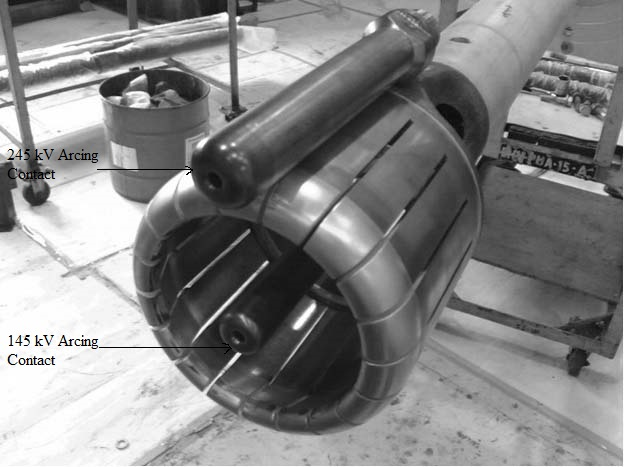
\includegraphics[width=\textwidth]{WrongAssemblyofArcingContact}
    \caption{Wrong Assembly of Arcing Contact}
    \label{fig:Wrong Assembly of Arcing Contact}
\end{figure}

\subsubsection*{Case no. 3}
The no load opening graph of a 245 kV SF\textsubscript{6} CB during closing was normal as observed in figure \ref{fig:Closing Graph of 245 kV SF6 Circuit Breaker}. But contact bouncing and current breaking in the closing part of the DCRM (Figure \ref{fig:Complete DCRM Signature of 245 kV SF6 Circuit Breaker}) was seen. The DCRM in the tripping portion is shown in figure \ref{fig:DCRM of 245 kV SF6 Circuit Breaker in Tripping Zone}. The closing operation was repeated, and bouncing was seen in the closing graph (Figure \ref{fig:Contact Bouncing in Closing Graph of 245 kV SF6 Circuit Breaker}). The interrupter was opened, and it was observed that moving arcing contact was become loose. The required tightening torque was not applied during assembly. In consequent mechanical operations, it started becoming more and more loose. After rectification of the problem, the normal signature was obtained.

\begin{figure}[!htbp]
    \centering
    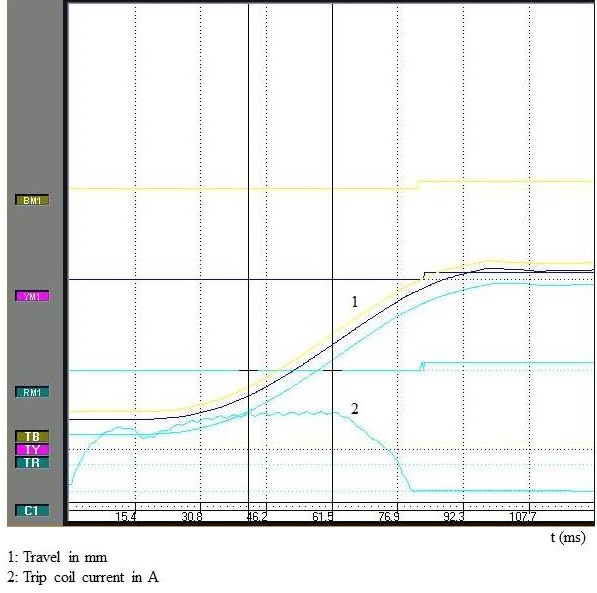
\includegraphics[height=4in]{ClosingGraphof245kV}
    \caption{Closing Graph of 245 kV SF\textsubscript{6} Circuit Breaker}
    \label{fig:Closing Graph of 245 kV SF6 Circuit Breaker}
\end{figure}

\begin{figure}[!htbp]
    \centering
    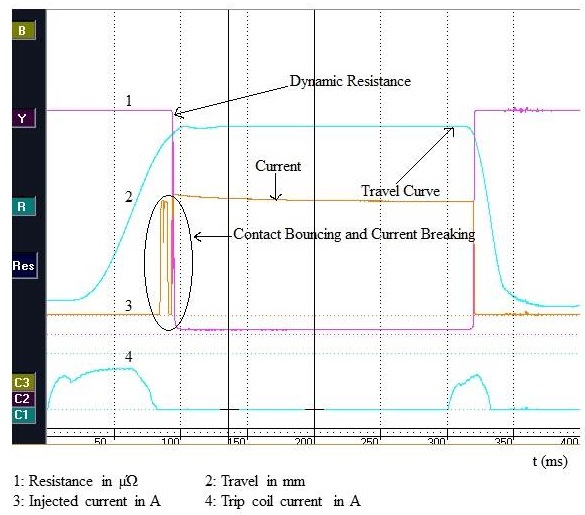
\includegraphics[height=4in]{CompleteDCRMSignatureof245}
    \caption{Complete DCRM Signature of 245 kV SF\textsubscript{6} Circuit Breaker}
    \label{fig:Complete DCRM Signature of 245 kV SF6 Circuit Breaker}
\end{figure}

\begin{figure}[!htbp]
    \centering
    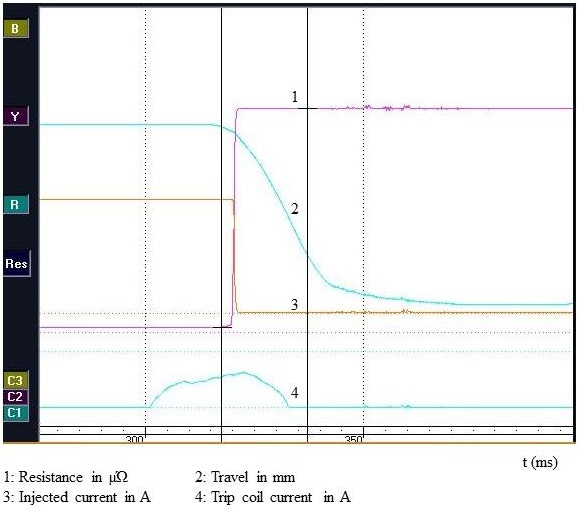
\includegraphics[height=4in]{DCRMof245kVSF6}
    \caption{DCRM of 245 kV SF\textsubscript{6} Circuit Breaker in Tripping Zone }
    \label{fig:DCRM of 245 kV SF6 Circuit Breaker in Tripping Zone}
\end{figure}

\begin{figure}[!htbp]
    \centering
    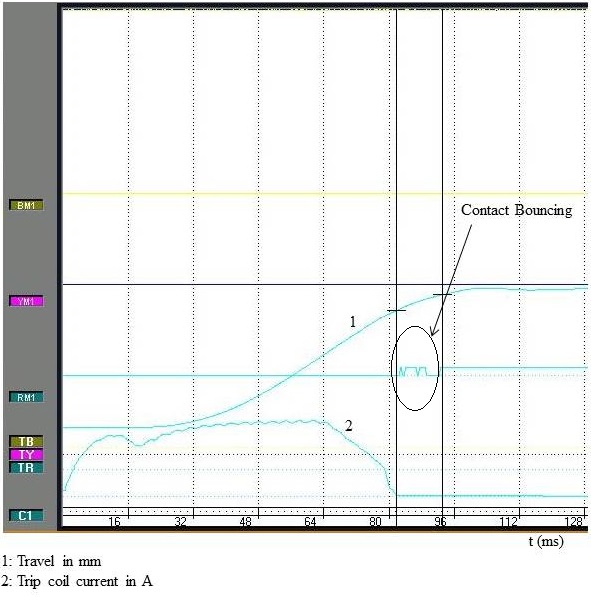
\includegraphics[height=4in]{ContactBouncinginClosingGraph}
    \caption{Contact Bouncing in Closing Graph of 245 kV SF\textsubscript{6} Circuit Breaker}
    \label{fig:Contact Bouncing in Closing Graph of 245 kV SF6 Circuit Breaker}
\end{figure}
\clearpage

\subsubsection*{Case no. 4}
Contact resistance measurement of a 220 kV SF\textsubscript{6} CB used for switching 220/33 kV, 50 MVA transformer in 400 kV substation, Waluj, Aurangabad showed a high value of resistance of the order of 200 kΩ for R-pole. The measurement test was repeated, and it was showing higher values. After repeated tests, the result was found to be higher value for resistance. DCRM test was conducted. A lot of fluctuations were observed in the resistance in no action zone of the DCRM signature as shown in figure \ref{fig:Abnormal Variations in Resistance in no Action Zone of DCRM Signature for 220 kV Circuit Breaker}. DCRM test was repeated again after confirming the connections. No change was observed in the signature. It was decided to open the R-pole. It was observed that the ring connecting the PTFE nozzle of the main contact became loose. Scratch marks were also found as seen in figure \ref{fig:Loose Ring Connecting PTFE Nozzle of Main Contact}. The signature was normal after attending the problem.

\begin{figure}[!htbp]
    \centering
    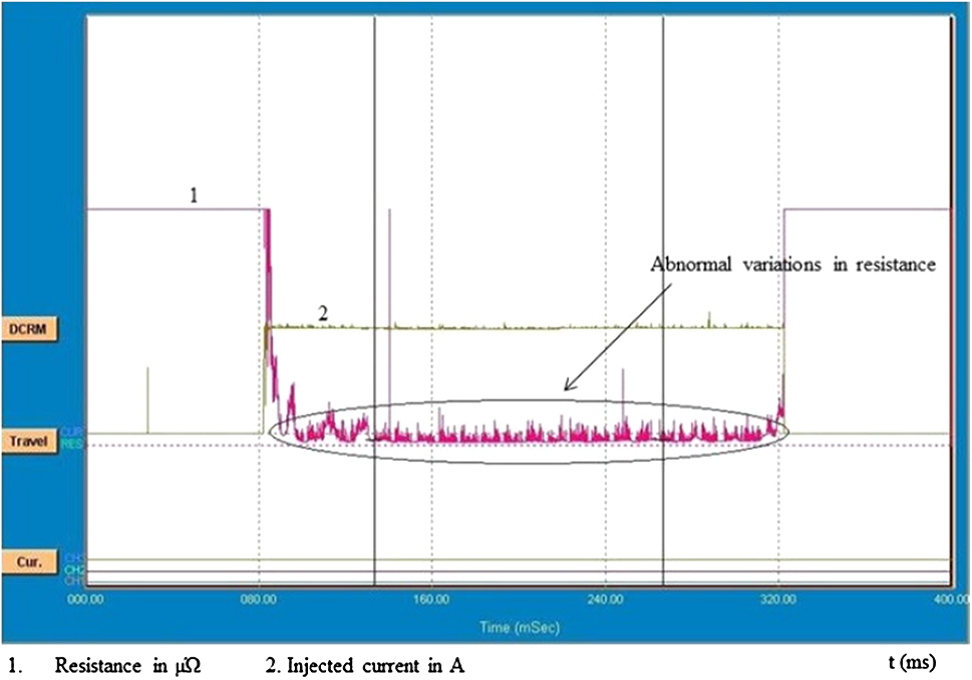
\includegraphics[width=\textwidth]{AbnormalVariationsinResistanceinno}
    \caption{Abnormal Variations in Resistance in no Action Zone of DCRM Signature for 220 kV Circuit Breaker}
    \label{fig:Abnormal Variations in Resistance in no Action Zone of DCRM Signature for 220 kV Circuit Breaker}
\end{figure}

\begin{figure}[!htbp]
    \centering
    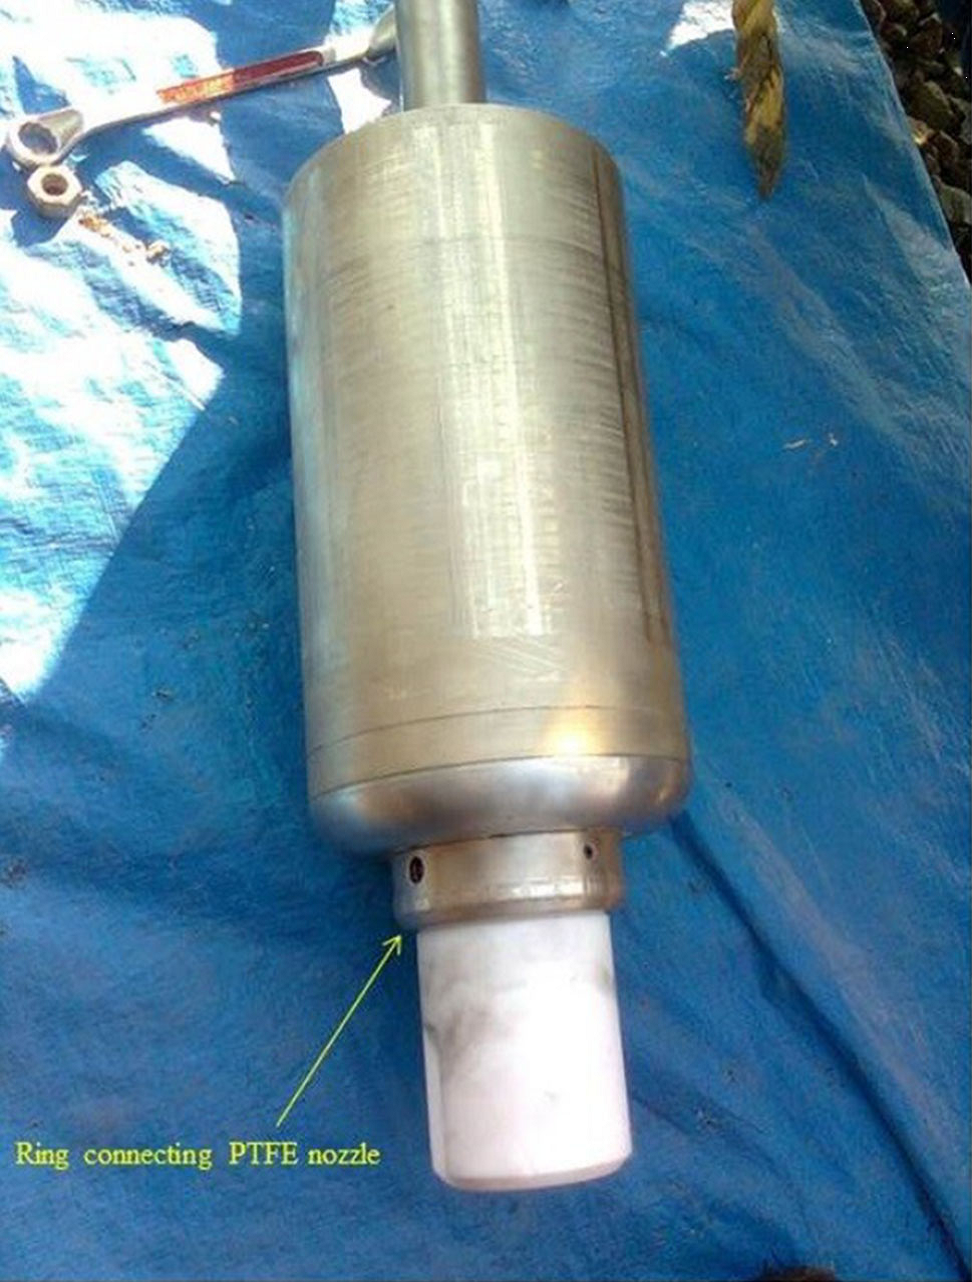
\includegraphics[height = 4in]{LooseRingConnectingPTFE}
    \caption{Loose Ring Connecting PTFE Nozzle of Main Contact}
    \label{fig:Loose Ring Connecting PTFE Nozzle of Main Contact}
\end{figure}

\subsubsection*{Case no. 5}
Abnormal peak in the DCRM signature in the close zone portion of a 400 kV CB was seen in after three years of installation. The static contact resistance was found be 150 $\mu \Omega$. The CB was opened for contact inspection. Following observations were made.

\begin{enumerate}
\item This breaker has seen more fault operations and high current making and breaking operations

\item Due to arcing between contacts in SF\textsubscript{6} gas environment metal fluorides and metal sulfates were formed inside arcing chamber which increased the resistance to considerable value

\item Because of high temperature attained during arcing, finger contacts of moving arc contact got expanded and contact burning at both side caused abnormal DCRM

\item Because of early detection of faulty internal condition through DCRM testing, major failure is avoided
\end{enumerate}

Figures \ref{fig:Problematic DCRM Signature} to \ref{fig:Deposition of Sulfide Powder on Contact Assembly} indicates the signature and internal contact conditions of the CB.

\begin{figure}[!htbp]
    \centering
    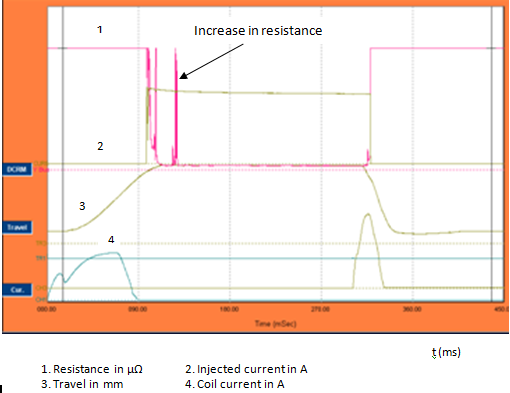
\includegraphics[width=0.8\textwidth]{ProblematicDCRMSignature}
    \caption{Problematic DCRM Signature}
    \label{fig:Problematic DCRM Signature}
\end{figure}

\begin{figure}[!htbp]
    \centering
    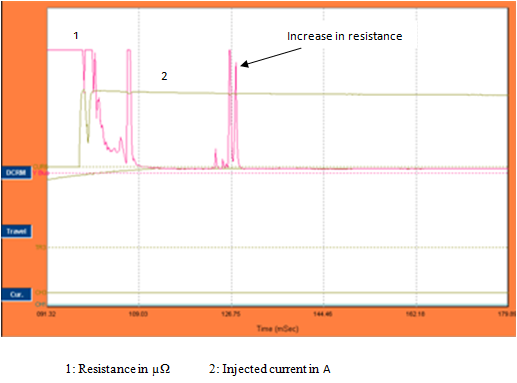
\includegraphics[width=0.8\textwidth]{IncreaseinResistanceinCloseZone}
    \caption{Increase in Resistance in Close Zone}
    \label{fig:Increase in Resistance in Close Zone}
\end{figure}
%*************************************************************
%\begin{figure}
%    \centering
%    \begin{subfigure}[b]{0.3\textwidth}
%        \centering
%        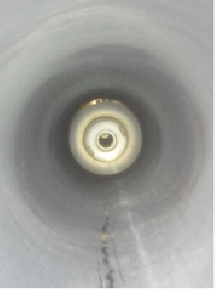
\includegraphics[width=\textwidth]{i1Movingcontactassemblyinside}
%        \caption{Moving contact assembly inside porcelain}
%        \label{fig:Moving contact assembly inside porcelain}
%    \end{subfigure}
%
%    \begin{subfigure}[b]{0.3\textwidth}
%        \centering
%        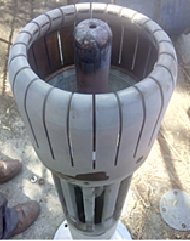
\includegraphics[width=\textwidth]{i2Stationarycontactassembly}
%        \caption{Stationary contact assembly}
%        \label{fig:Stationary contact assembly}
%    \end{subfigure}
%    \\
%    \begin{subfigure}[b]{0.3\textwidth}
%        \centering
%        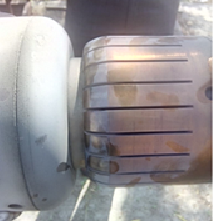
\includegraphics[width=\textwidth]{i3Fixedandmovingcontacts}
%        \caption{Fixed and moving contacts in engaged condition after removal from porcelain}
%        \label{fig:Fixed and moving contacts in engaged condition after removal from porcelain}
%    \end{subfigure}
%    
%    \begin{subfigure}[b]{0.3\textwidth}
%        \centering
%        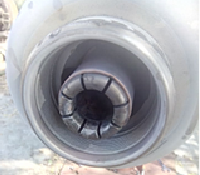
\includegraphics[width=\textwidth]{i4Movingcontactassembly}
%        \caption{Moving contact assembly after Teflon removal}
%        \label{fig:Moving contact assembly after Teflon removal}
%    \end{subfigure}
%    \\
%    \begin{subfigure}[b]{0.3\textwidth}
%        \centering
%        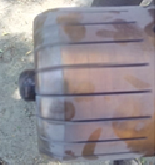
\includegraphics[width=\textwidth]{i5Fixedcontactassembly}
%        \caption{Fixed contact assembly}
%        \label{fig:Fixed contact assembly}
%    \end{subfigure}
%    
%    \caption{Fix and Moving Contact Assembly}
%    \label{fig:Fix and Moving Contact Assembly}
%\end{figure}
%***********************************************************************************
\begin{figure}
    \centering
    \begin{subfigure}[b]{0.3\textwidth}
        \centering
        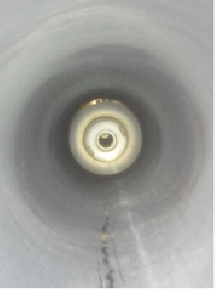
\includegraphics[width=\textwidth, height=6cm]{i1Movingcontactassemblyinside}
        \caption{Moving contact assembly inside porcelain}
        \label{fig:Moving contact assembly inside porcelain}
    \end{subfigure}
    \begin{subfigure}[b]{0.3\textwidth}
        \centering
        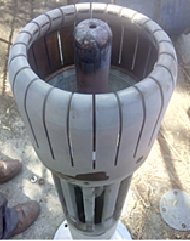
\includegraphics[width=\textwidth, height=6cm]{i2Stationarycontactassembly}
        \caption{Stationary contact assembly}
        \label{fig:Stationary contact assembly}
    \end{subfigure}
    \begin{subfigure}[b]{0.3\textwidth}
        \centering
        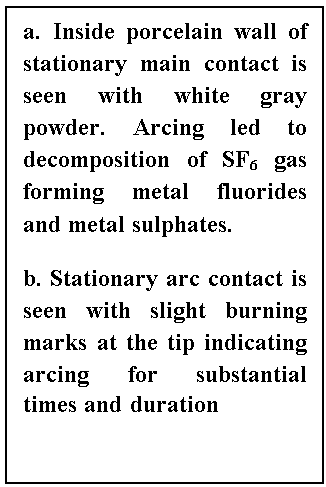
\includegraphics[width=\textwidth, height=6cm]{imInside}
        \vspace{0.9cm}
    \end{subfigure}
    \\
    \begin{subfigure}[b]{0.3\textwidth}
        \centering
        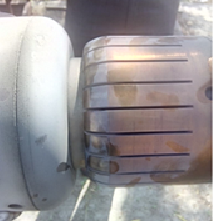
\includegraphics[width=\textwidth, height=5cm]{i3Fixedandmovingcontacts}
        \caption{Fixed and moving contacts in engaged condition after removal from porcelainn}
        \label{fig:Fixed and moving contacts in engaged condition after removal from porcelain}
    \end{subfigure}
    \begin{subfigure}[b]{0.3\textwidth}
        \centering
        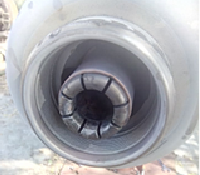
\includegraphics[width=\textwidth, height=5cm]{i4Movingcontactassembly}
        \caption{Moving contact assembly after Teflon removal}
        \label{fig:Moving contact assembly after Teflon removal}
        \vspace{0.7cm}
    \end{subfigure}
    \begin{subfigure}[b]{0.3\textwidth}
        \centering
        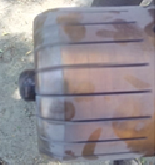
\includegraphics[width=\textwidth, height=5cm]{i5Fixedcontactassembly}
        \caption{Fixed contact assembly}
        \label{fig:Fixed contact assembly}
        \vspace{1.4cm}
    \end{subfigure}
    \caption{Fix and Moving Contact Assembly}
    \label{fig:Fix and Moving Contact Assembly}
\end{figure}

%***********************************************************************************
\begin{figure}
    \centering
    \begin{subfigure}[b]{0.49\textwidth}
        \centering
        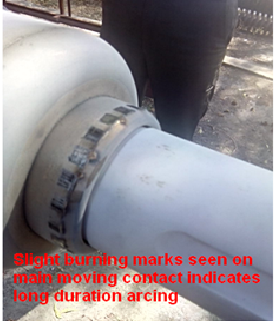
\includegraphics[width=\textwidth, height=7cm]{j1PufferCylinderSlidingContacts}
        \caption{Puffer Cylinder Sliding Contacts}
        \label{fig:Puffer Cylinder Sliding Contacts}
    \end{subfigure}
    \begin{subfigure}[b]{0.49\textwidth}
        \centering
        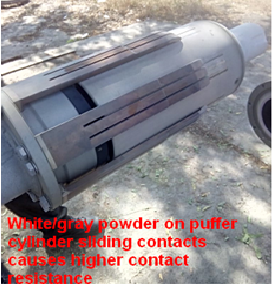
\includegraphics[width=\textwidth, height=7cm]{j2MainMovingContact}
        \caption{Main Moving Contact}
        \label{fig:Main Moving Contact}
    \end{subfigure}
    \\
    \begin{subfigure}[b]{0.49\textwidth}
        \centering
        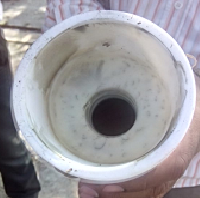
\includegraphics[width=\textwidth, height=6cm]{j3MovingArcContactSideofNozzle}
        \caption{Moving Arc Contact Side of Nozzle}
        \label{fig:Moving Arc Contact Side of Nozzle}
    \end{subfigure}
    \begin{subfigure}[b]{0.49\textwidth}
        \centering
        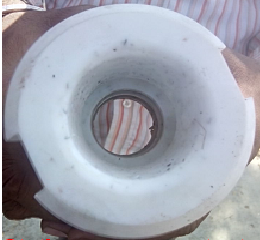
\includegraphics[width=\textwidth, height=6cm]{j4StationaryContactSideofNozzle}
        \caption{Stationary Contact Side of Nozzle}
        \label{fig:Stationary Contact Side of Nozzle}
    \end{subfigure}
    
    \caption{Deposition of Sulfide Powder on Contact Assembly}
    \label{fig:Deposition of Sulfide Powder on Contact Assembly}
\end{figure}

\clearpage
\section[New Algorithm for Contact Condition Detection of SF\textsubscript{6} CB]{New Algorithm for Contact Condition \\Detection of SF\textsubscript{6} CB}

Tests were conducted on 400 kV and 245 kV SF\textsubscript{6} CBs at circuit breaker manufacturing industry, 400 kV substation Waluj, Aurangabad and 765 kV substation at Thapti Tanda Aurangabad. Timing measurement, SCRM as well as DCRM tests were conducted. Data of DCRM for healthy breakers as well as breakers with problems in condition of contact was collected from the largest utility company PGCIL as well as MSETCL. Figure \ref{fig:DCRM Signature Showing the Parameters used in Algorithm} shows the DCRM signature in the tripping portion along with the parameters.

\begin{figure}[!htbp]
    \centering
    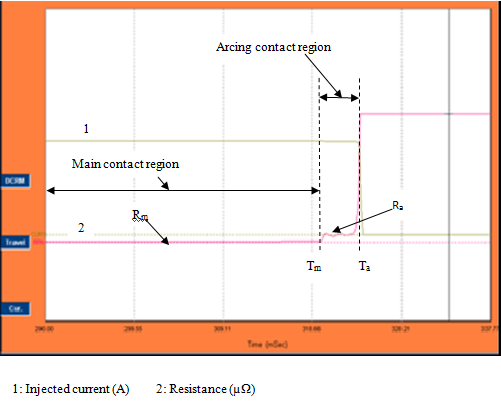
\includegraphics[width=\textwidth]{DCRMSignatureShowingtheParametersusedinAlgorithm}
    \caption{DCRM Signature Showing the Parameters used in Algorithm}
    \label{fig:DCRM Signature Showing the Parameters used in Algorithm}
\end{figure}

Following parameters are used for developing contact wear algorithm:

$T_m$ - time at the position when main contact disengages (ms)\\
$T_a$ - time at the position when arc contact disengages (ms)\\
$R_{aimax}$ - arc contact resistance at the point of main contact disengagement ($\mu \Omega$)\\
$A_m$ - area below the main contact resistance zone ($\mu \Omega \times$ms)\\
$A_a$ - area under the arc contact zone ($\mu \Omega \times$ms)\\
$R_m$ - average contact resistance in the main contact region ($\mu \Omega$)\\
$R_a$ - average contact resistance in the arc contact region ($\mu \Omega$)

Deviations in the above parameters from the healthy DCRM signature will be used for developing the contact wear algorithm. Number of DCRM signatures was analyzed and following observations are made. 

\subsubsection*{Fixed arc contact tip wear}
Over the times due to arcing and heat, length of fixed arc contact reduces. Shortening of fix arc contact will be reflected at the end of the resistance curve during tripping portion. Position at which the arc contact disengages finally will shift to left than normal curve. Average arc contact resistance will increase, but the area below the DCRM curve in arc contact zone will decrease due to earlier disengagement of arc contact. Since main contact condition is sound, the point at which main contact disengages will remain same so also the area below the main contact resistance zone. In this case, the motion will start earlier than in previous measurement indicating wearing of contact.$\Delta T_m = 0, \Delta T_a < 0, \Delta A_a < 0, \Delta R_{aimax} = 0$ and $\Delta A_m = 0$. Arcing contact wipe will decrease.

\subsubsection*{Wearing of moving arc contact}
Excessive heat and arcing also damage the fingers of arc contact. Damage to fingers will increase the initial resistance of the arc contact at the point of disengagement of the main contact. As the fix arc contact is assumed to be sound, the position of arc contact disengagement will remain same. The area under the arc contact zone will increase. This will lead to the conditions $\Delta T_m = 0, \Delta T_a = 0, \Delta A_a > 0, \Delta R_{aimax} > 0$ and $\Delta A_m = 0$. Erosion of the moving arc contact will increase the resistance in the arc contact zone.

\subsubsection*{Main contact erosion}
If the force of the fingers of the main contact is not proper or the contacts are not aligned properly, or the tightening torque is not applied then the main contact may erode. This will not change the position of arc contact disengagement but will certainly change the point of main contact disengagement. This will slightly increase the area below the arc contact zone. Variations in the no action zone of the DCRM will be seen which will increase the average main contact resistance. Increase in resistance during static contact resistance measurement can also be observed. The condition will be $ \Delta T_m < 0, \Delta A_a > 0, \Delta T_a = 0, \Delta R_{aimax} = 0, \Delta A_m > 0$.

\subsubsection*{Arc contact (fixed and moving) and main contact erosion}
Erosion of fixed arc contact and main contact will change both the position of main and arc contact displacement resulting in reduction in area below the arc contact region and increasing the arc contact resistance at the disengagement of main contact resistance position at the same time variations in the close portion of the DCRM is also observed increasing the area below the main contact resistance zone. Arcing contact wipe will be reduced leading to a condition of $ \Delta T_m < 0, \Delta T_a < 0, \Delta A_a < 0, \Delta R_{aimax} > 0, \Delta A_m >0$.

\subsubsection*{Fix and Moving arc contact erosion}
Excessive arcing and heating may shorten the fixed arc contact at the same time melting at the fingers of moving contact may happen over the years due to switching of short circuit currents or frequent capacitor switching. This condition can be identified as $\Delta A_a < 0, \Delta T_a < 0, \Delta T_m = 0, \Delta R_{aimax} > 0$ and $ \Delta A_m = 0 $.

Based on the analysis of field DCRM, an algorithm is proposed for detecting the contact wear. Deviations in the DCRM signature from normal values are the input to the algorithm. Five parameters, deviation in the main contact cut off time ($\Delta T_a$), arcing contact cut off time ($\Delta T_a$), area below the curve in arc contact zone ($\Delta A_a$), arc contact resistance at the point of main contact disengagement ($\Delta R_{aimax}$) and the area below the curve in main contact zone ($\Delta A_m$) are used. Following cases of contact erosion is identified:
\clearpage

\begin{description}
\item[Problem 1:] Main contact erosion
\item[Problem 2:] Fix arcing contact erosion
\item[Problem 3:] Wearing of arcing contact fingers
\item[Problem 4:] Fix and Moving arcing contact erosion
\item[Problem 5:] Arcing contact (Fix and Moving) and main contact erosion
\end{description}

%************* Three Page Figure*****************************************
\begin{figure}[!ht]
\centering
    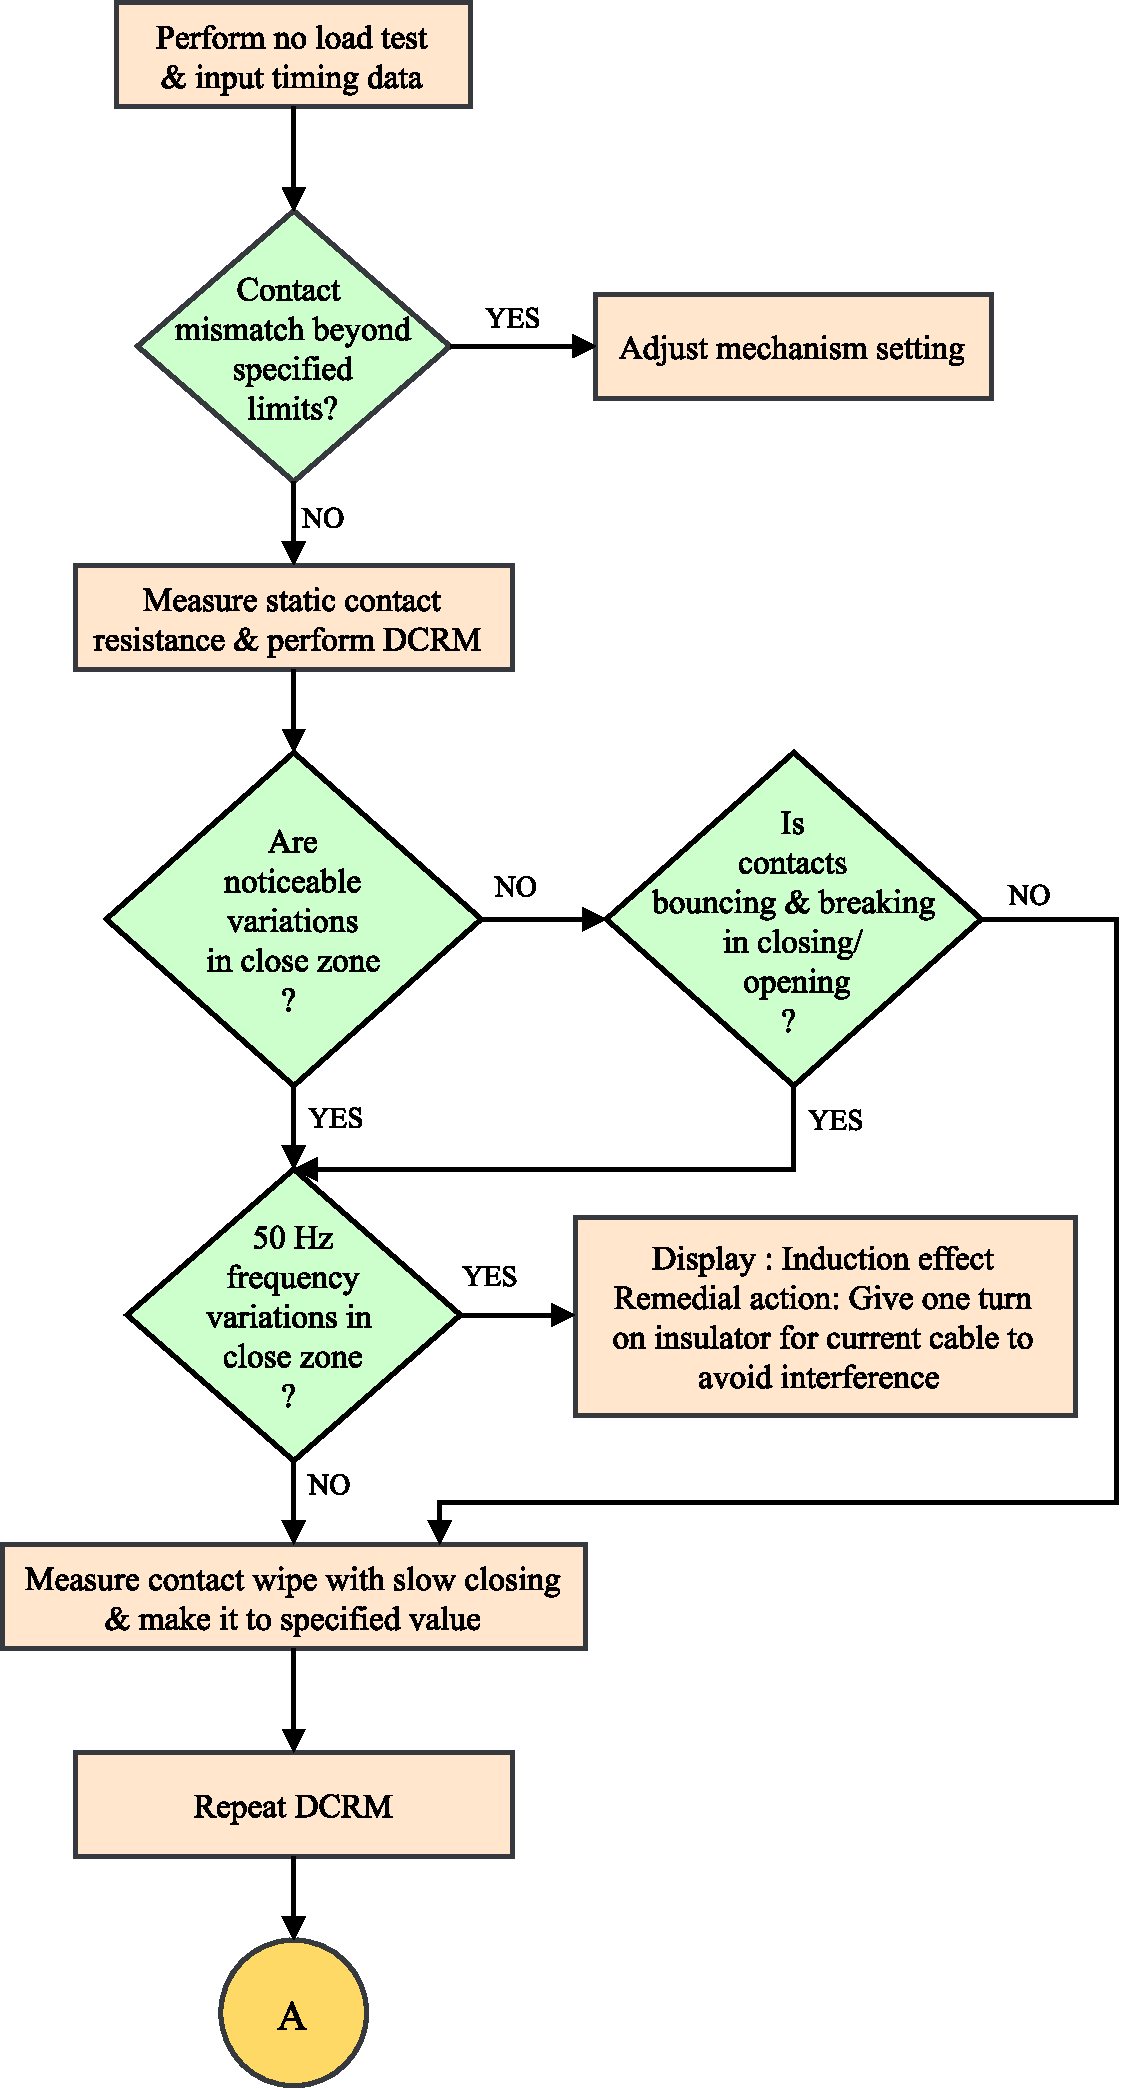
\includegraphics[width=\textwidth, height=9.69in ]{FlowChartofProposedAlgorithm1}
\end{figure}
\begin{figure}[!ht]
\centering
    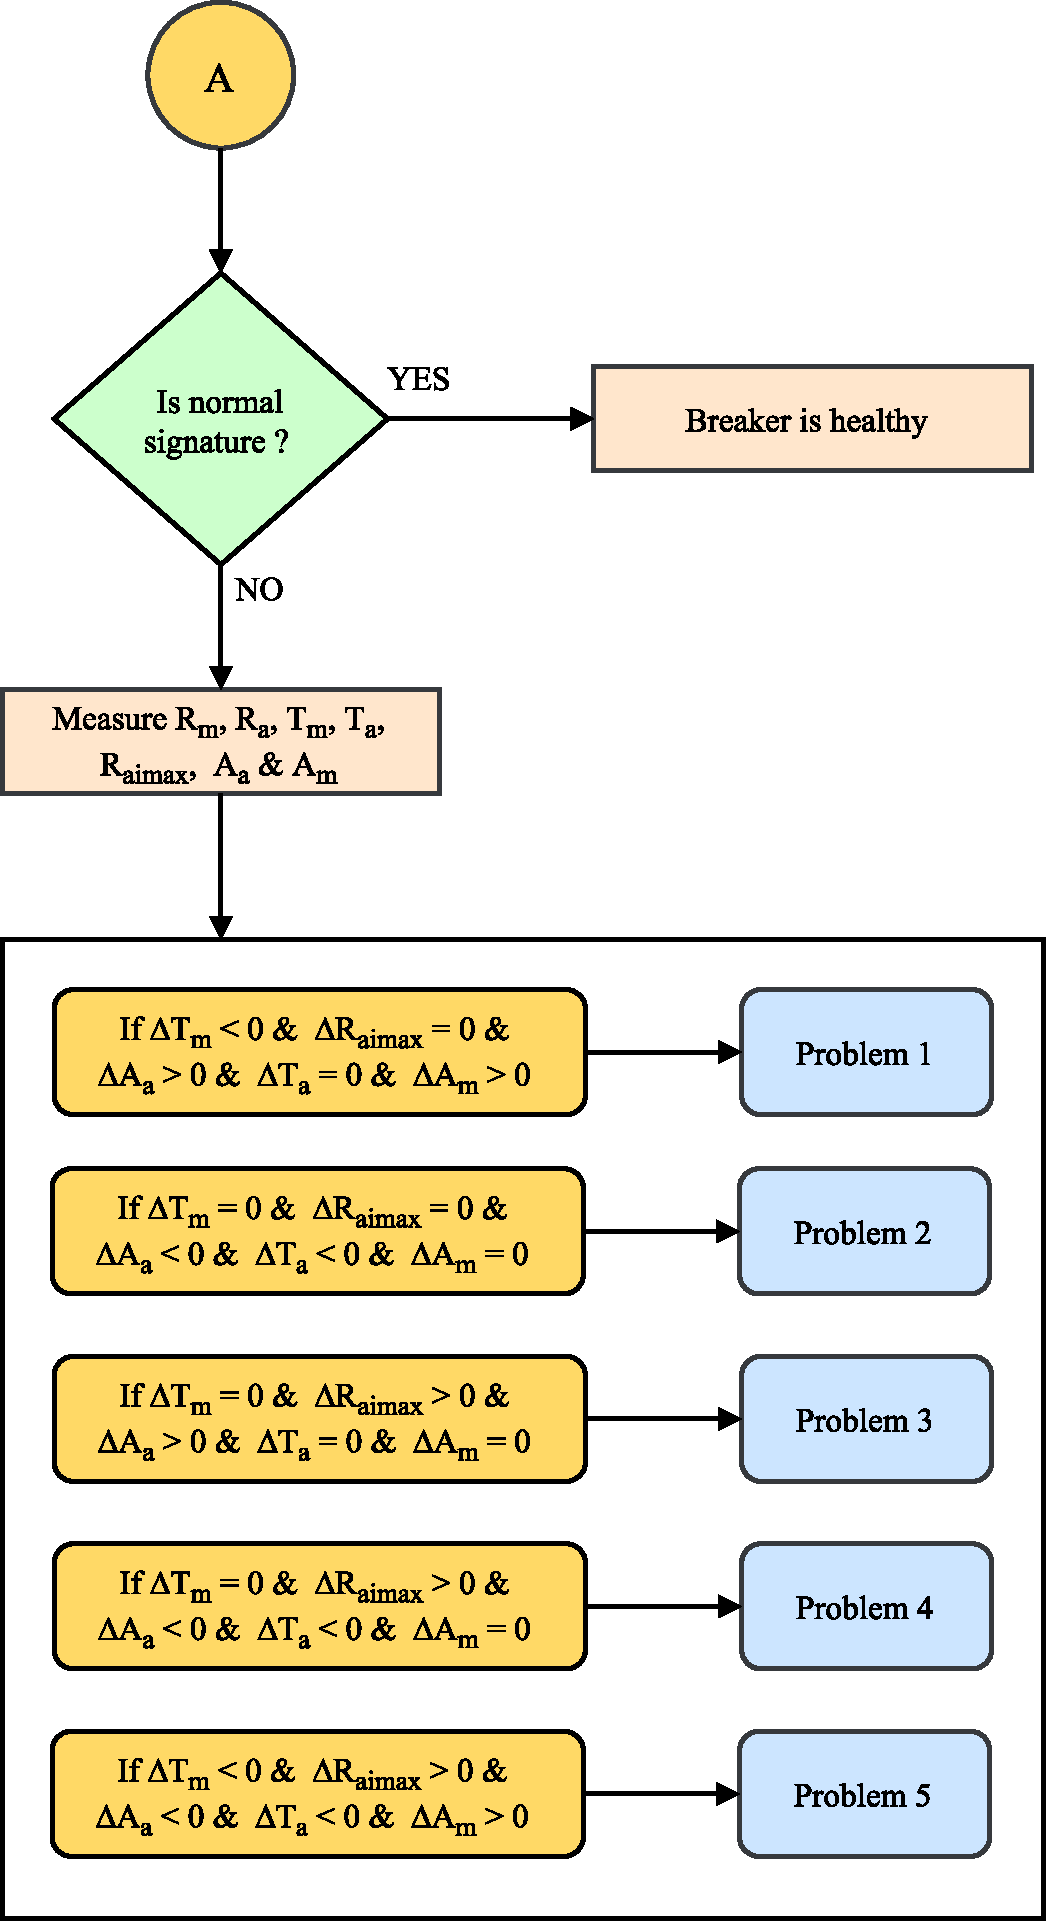
\includegraphics[width=\textwidth, height=9.69in]{FlowChartofProposedAlgorithm2}
\end{figure}
\clearpage
\begin{figure}[H]
    \centering
    \begin{tabular}{| c | l |}
	\hline
	\textbf{Problem} & \multicolumn{1}{|c|}{\textbf{Description}} \\ \hline
	1					& Main contact erosion \\ \hline
	2					& Fix arcing contact erosion \\ \hline
	3					& Wearing of arcing contact fingers \\ \hline
	4					& Fix and moving arc contact erosion \\ \hline
	5					& Arc contact (Fix and moving) and main contact erosion\\ \hline
	\end{tabular}
    \caption{Flow Chart of Proposed Algorithm}
    \label{fig:Flow Chart of Proposed Algorithm}
\end{figure}

Figure \ref{fig:Flow Chart of Proposed Algorithm} shows the flow chart for the proposed algorithm. A program is developed in Java which depicts the health of CB.
%***************************************************************************

%\begin{tabular}{| >{\arraybackslash}m{1.9in} |>{\centering\arraybackslash}m{0.6in} |>{\arraybackslash}m{2.75in} |}

